\chapter{Introduction and literature review} \label{sec:intro}


\section{General introduction}

The liminal space between biology and physics is perhaps nowhere more salient than in the study of electrophysiology, where the emergent properties that characterize life intersect with the fundamental laws of nature. This intersection is certainly most profound in the microscopic details of the brain where cognition and consciousness emerge from electric fields. Our ability to measure these electrical signals through unit and field recordings or by proxy through calcium imaging lets us dissect the physical implementations of animal behaviour. To the benefit of science and medicine, these electric fields can also be recorded non-invasively from humans using scalp electrodes.

Despite the coarseness of its measurements, the electroencephalogram (EEG) has proven itself to be highly useful. EEG studies of human subjects benefit from being able to associate brain signals with complex cognitive paradigms such as memory \cite{Osipova2006, Sauseng2009, Sauseng2010}, perception \cite{Rodriguez1999, Melloni2007,Fahrenfort2012}, and attention \cite{Hillyard1998, Makeig2002}, which are more difficult to perform and assess with animals. The ability to measure brain activity relatively cheaply and easily has also made EEG a fecund source of neuromarkers for neurological conditions and brain states, most notably epilepsy \cite{Engel1984,Noachtar2009} and sleep \cite{Wolpert1969, Prerau2016}. Its modern clinical applications have been extended to include monitoring depth of anesthesia \cite{Michael2008} and detecting brain ischemia \cite{Meghdadi2021}, while ongoing research is trying to use EEG to predict various neurological conditions, including autism \cite{Bosl2018}, dementia \cite{Meghdadi2021}, schizophrenia \cite{Meghdadi2021}, and depression \cite{DeAguiarNeto2019}. Outside the clinic, advances in wearable EEG technology has lead to its growing commercial use in brain-machine interfaces \cite{Mahmood2021} and biofeedback technology \cite{Hunkin2021}. 

After a century of EEG recordings \cite{Berger1929}, a lot still remains unknown about what these signals actually reflect about the brain \cite{Cohen2017}, especially when compared to invasive measurements like single unit recordings. However, as the neurophysiological basis of EEG is elucidated, its valuable correlates to cognition, disease, and states of consciousness can be mapped onto its neural substrate and further interrogated in animal models --- this connection is an important translational axis for brain research \cite{da2013eeg}. A fair amount of success has come from investigating synchronous neural oscillations, which generate rhythms on the EEG and whose neural basis can be studied in both mice and monkeys \cite{Buzsaki2004}. Building on this work, recent studies have begun identifying and quantifying \textit{broadband} components of EEG signals and correlating these features, such as the slope of the power spectrum (\autoref{fig:phenomenology}A), with cognitive tasks \cite{Ouyang2020,Podvalny2015,He2010,Waschke2021}, age \cite{Voytek2015}, neurological disease \cite{Wang2022, Pertermann2019, Schaworonkow2021, OSTLUND2021100931, MOLINA2020562, Robertson2019, Roche2019}, and various states of consciousness \cite{Colombo2019, Stock2020, Lendner2020, MUTHUKUMARASWAMY2018582}. In contrast to the classically considered narrowband oscillations, however, broadband EEG features remain poorly defined and their neurophysiological basis is both undetermined and controversial. 

\begin{figure}[b!]
    \centering
    \includegraphics[width=\textwidth]{Figures/chapter1/spectral_trend.pdf}
    
    \caption{\textbf{Example spectra illustrating the broadband characteristics of EEG.} 
    (\textbf{A}) Average EEG power spectrum during eyes closed, showing a slope in log-log space of $-1.32$. Data re-plotted from Pritchard \cite{Pritchard1992}. (\textbf{B}) Spectrum of \qty{83}{\minute} electrocorticographic signal of awake subject from three different electrodes, collected by He et al.\cite{He2010}.  (\textbf{C}) Changes in EEG spectrum under various conditions reported by Colombo et al.\cite{Colombo2019}. Panel B is reprinted with minor formatting changes from Neuron, 66/3, Biyu J. He, John M. Zempel, Abraham Z. Snyder, Marcus E. Raichle, The Temporal Structures and Functional Significance of Scale-free Brain Activity, 353-369, Copyright (2010), with permission from Elsevier. Panel C is adapted with minor formatting changes from Colombo et al. \cite{Colombo2019} under a Creative Commons license. © 2019 Colombo et al (CC BY-NC-ND 4.0).
    } 
    \label{fig:phenomenology}
\end{figure}

\section{Broadband EEG features and the spectral trend} \label{sec:phenomenon}
\subsection{Early characterization of broadband EEG}
Despite the relatively recent interest in broadband EEG, the fact that EEG signals exhibit broadband characteristics was noted in 1938 in the very first publication showing EEG spectra \cite{Grass1938}, which was computed with a mechanical apparatus of various wheels and projectors to transform the EEG output into Fourier space. If EEG signals were purely rhythmic, the spectrum should have shown discrete spectral peaks in narrow frequency bands corresponding to each of several possible rhythmic components. However, what the authors observed was a continuum of power across a broad range of frequencies, i.e., a broadband signal. Based on these spectra, the authors noted that ``inspection of such continuous spectrums should convince one of the inadvisability of referring to certain potentials as alpha, beta, delta waves, etc.''\cite{Grass1938}. Inadvisable or not, this practice is still very much the norm today. After the introduction of computer analysis in the 1960s, EEG spectra became more routinely examined, but the broadband components of these spectra were only ever mentioned in passing \cite{Boudreau1963}. It was the prevailing view that the aim of EEG spectral analysis was the ``disclosure of sinusoidal periodicities buried in the random background activity'' \cite{Freeman1975}. 

In 1992, Pritchard \cite{Pritchard1992} published the first paper that considered the broadband properties of EEG signals as a feature in its own right. In his paper, Pritchard posited that EEG spectra exhibit power law scaling, i.e., $P\sim1/f^\beta$, with an exponent of $\beta=1.32$ (\autoref{fig:phenomenology}A) and used this to argue that the brain is fractal in nature~\footnote[2]{The spectral exponent is equivalent to the slope of the spectrum in log-log space. The phrase spectral exponent and spectral slope are therefore used interchangeably.}. This claim effectively kickstarted multiple competing theories on the origin and meaning of the background EEG spectrum (\autoref{sec:theories}). A later study by He et al. \cite{He2010} was the first to show explicitly that the spectral trend may disclose information about the brain and is not just noise to be ignored. Using a technique based on fractal theory, the authors separated out the rhythmic and $1/f$ fractal component of their signals, and showed that the spectral exponent changed with task performance \cite{He2010}. A plot of their data showing a spectrum from 0.01 to 100 \unit{\hertz} is shown in \autoref{fig:phenomenology}B and clearly illustrates how spectral peaks from brain rhythms seem rise up out of a background spectral trend. A plot from a more recent paper \cite{Colombo2019} is shown in \autoref{fig:phenomenology}C to illustrate how the background spectral trend can change depending on brain state. In sum, the broadband component of EEG signals is characterized by the overall background trend observed in EEG spectra. From the original paper by Pritchard \cite{Pritchard1992}, estimating power laws from this trend has been of particular interest to the field, and changes in the spectral exponent have since been correlated with myriad behavioural and neurological variables.

\subsection{Relevance for studying brain rhythms} \label{sec:detrending}
Having a physiological explanation for the spectral trend is obviously important for interpreting results like those in \autoref{fig:phenomenology}C. Why is the slope of the spectrum changing?
Additionally, a physiological interpretation of the spectral trend is important for studying the rhythmic component of EEG. Typically, the spectral trend is dealt with in one of several ways. By far the most common approach is to divide EEG spectra by the spectrum during a baseline condition. In cases that the spectral trend does not change, this technique removes the trend from the analysis. However, if the spectral trend changes between the conditions, e.g., \autoref{fig:phenomenology}C, this technique assumes that any change in a given frequency band is caused by differences in brain rhythms \cite{Gerster2022}.

Those who argue for a deeper meaning behind the spectral trend have developed EEG analyses that deal with the spectral trend explicitly. The first of these procedures is to ``whiten'' the spectrum by fitting and removing the spectral trend prior to analyzing changes in brain rhythms \cite{Buzsaki2004,Buzsaki2006,Donoghue2020}. A popular algorithm for fitting the spectral trend, called FOOOF \cite{Donoghue2020}, models the spectral peaks as Gaussian functions multiplied by a $1/f^\beta$ trend. In other words, this technique assumes that the spectral trend follows a power law and accounts for this power relationship when measuring brain rhythms. A less common technique is to recompute the EEG spectrum at different sampling frequencies. This is supposed to separate narrowband oscillations from any fractal component of the data, which due to the self-similar nature of fractals is invariant under temporal rescaling \cite{Yamamoto1993}. An algorithm based on this technique has been developed, called Irregular-Resampling Auto-Spectral Analysis (IRASA) \cite{Wen2016}. This analysis makes the specific assumption that the spectral trend reflects fractal brain activity and should be removed from brain rhythm estimates.

\begin{wrapfigure}[15]{r}{80mm}
\vspace{-15pt}
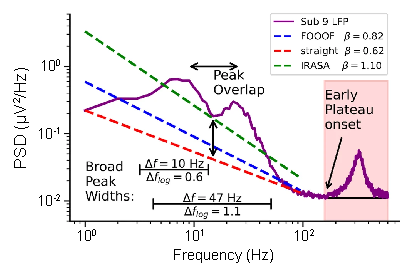
\includegraphics[width=75mm]{Figures/chapter1/gerster.pdf}
\vspace{-10pt}
\caption{ \captiontitle{Difficulties of estimating spectral exponents with various methods.} The spectrum of a macroscopic neural recording (purple), analyzed with three methods to estimate the spectral exponent, including FOOOF (blue line), IRASA (green line), and basic linear regression (red line). These methods give different values for $\beta$ (see legend). Above \qty{100}{\hertz}, the spectral trend plateaus. Figure modified from Gerster et al. \cite{Gerster2022} under a Creative Commons license. © 2022 Gerster et al (CC BY 4.0).
} \label{fig:gerster}
\end{wrapfigure}

Clearly these last two methods will lead to very different conclusions compared to a traditional baseline-normalized analysis. In fact, these last two methods produce different outcomes from \textit{each other} when applied to the same spectrum (\autoref{fig:gerster}). This inconsistency comes from lacking a unified, physiological definition of broadband EEG. Furthermore, at higher frequencies, spectra typically exhibit a plateau  (\autoref{fig:gerster}) whose origin and interpretation remain unresolved \cite{Gerster2022}. The techniques above do not provide a systematic approach to dealing with this part of the spectral trend other than restricting the frequency range of analysis. This limitation illustrates that, while prevalent, the power-law scaling description of EEG spectra does not capture the full broadband nature of EEG signals. 

In summary, every analysis procedure makes some assumption about the spectral trend which affects the interpretation of both the broadband and rhythmic components of EEG. Ignoring the trend makes the specific assumption that it should be included in brain rhythms estimates. Deciding to remove it requires a quantitative definition for the spectral trend and its interaction with brain rhythms. Currently, different studies use different methods for spectral analysis and may therefore interpret the same data in distinct ways. Moreover, many of the theories on the spectral trend do not yet have quantitative methods associated with them, and thus the methodologies described above only reflect a subset of the existing interpretations of broadband EEG --- all of which will be reviewed in detail later.

\subsection{Summary}
The past three decades have seen an increasing awareness that EEG exhibits broadband characteristics which change with task performance and brain state. This feature is most often described as a $1/f^\beta$ scaling of the EEG spectrum and analysis technique have been developed to estimate the spectral exponent, $\beta$, as well as to correct for the spectral trend when estimating brain rhythms. However, without a complete understanding of the mechanism(s) giving rise to the broadband characteristics of EEG, interpreting differences in the spectral trend has been speculative and the veracity of detrended EEG analyses has remained debatable. Understanding the neurophysiological basis of the EEG spectral trend is the central aim of this thesis, with the view that a comprehensive explanation of the spectral trend will improve interpretation and analysis of EEG data. In the main chapters, I will present biophysical modelling results that describe how neurophysiological systems might generate broadband EEG signals. In the next sections of this chapter, I provide background for the modelling work in this thesis with an overview of the biophysics and neural basis of EEG, before finally reviewing existing theories on the origin of the EEG spectral trend.

\section{The biophysics of EEG} \label{sec:EM_theory}

A strength of EEG and electrophysiological measurements in general is that the biophysics of these measurements are understood. In this section, I review the basics of electromagnetism in a volume conductor and build up to forward models of the EEG --- models that take a distribution of currents in the brain and give as an output the electric potential at the scalp.

\subsection{Maxwell's equations and the electric potential}
In 1873, James Clerk Maxwell published his treatise on electricity and magnetism, accomplishing for electromagnetism what Newton had for mechanics. In four equations, the behaviour of all classical phenomena related to electricity and magnetism could be described. As such, they are the basic laws that turn physiology into \textit{electro}physiology. The equations are
\begin{align*}
    & \nabla \cdot \bm{E} = \frac{\rho}{\epsilon_0} \\
    & \nabla \cdot \bm{B} = 0 \\
    & \nabla \times \bm{E} = - \frac{\partial {B}}{\partial t} \\
    & \nabla \times \bm{B} = \mu \left( \bm{J} + \epsilon_0 \frac{\partial \bm{E}}{\partial t} \right)
\end{align*}
Here, $\bm{E}$ is a vector field called the electric field and $\bm{B}$ is a vector field called the magnetic field. The first two equations describe the divergence of these fields and the latter two equations describe the curl of these fields. 

The first equation states that the sources (positive divergence) and sinks (negative divergence) of the electric field are electric monopoles, otherwise called an electric charge. $\rho$ is the density of charge at each point in space and when scaled by $\epsilon_0$, the permittivity of a vacuum, one gets the divergence of the electric field. Negative charges are sinks of the electric field and positive charges are sources of the electric field. The second equation states that there are no source or sinks of the magnetic field. In other words, there are no magnetic monopoles. The third and fourth equation describe how the electric and magnetic field interact with each other. The third equation is called Faraday's law of induction and describes how a time varying magnetic field can induce an electric field. The final equation is Ampère's law and describes how a magnetic field is generated by either an electric current or a time varying electric field.

\subsubsection{The quasi-stationary approximation of the electric potential}
In EEG, the electromagnetic field is assumed to be static which is called the quasi-stationary approximation \cite{Plonsey1967}. This approximation is valid because the frequencies of EEG we are interested in (less than \qty{1}{\kilo\hertz}) are slow compared to the timescale of interactions between the electric and magnetic fields \cite{RevModPhys.65.413}. As a result of the assumption, all the time derivatives in the equations are zero, reducing Maxwell's equations to
\begin{align}
    & \nabla \cdot \bm{E} = \frac{\rho}{\epsilon_0} \\
    & \nabla \cdot \bm{B} = 0 \\ 
    & \nabla \times \bm{E} \approx 0 \label{eq:QSA_induction} \\ 
    & \nabla \times \bm{B} \approx \mu \bm{J} \label{eq:QSA_amp_law}
\end{align}
Notice that the electric field has become uncoupled from the magnetic field. This assumption allows for valid and (relatively) simple calculations of the electric potential at the scalp.

\subsubsection{Calculating the electric potential at the scalp}
EEG electrodes measure the electric potential, $\phi$, at a location on the scalp. The electric potential of an electric field is defined by the fundamental theorem of vector calculus: $\bm{E} = - \nabla \phi + \nabla \times \bm{A}$, where $\bm{A}$ is some divergence-free vector field. Under the quasi-stationary approximation, the electric field has no curl (\ref{eq:QSA_induction}), and thus $\nabla \times \bm{A}$ must equal zero, simply giving us that 
\begin{equation} \label{eq:potential}
\bm{E} = -\nabla \phi
\end{equation}
This equation tells us that the electric field is entirely defined by the gradient of the electric potential. We can therefore calculate the electric potential from its relationship with the electric field. To do so, we make use of two additional relationships.

First, an electric field in a conductor acts on free charges and gives rise to a passive current, called the volume or return current, that obeys Ohm's law  \cite{RevModPhys.65.413}. That is, $\bm{J}^{v}(\bm{r}) = \sigma(\bm{r}) \bm{E}(\bm{r})$, where $\sigma$ is the macroscopic conductivity. This equation can be very general \cite{Pettersen2012}: $\sigma$ may be a tensor, meaning that the conductivity varies depending on the direction (anisotropy), it may be complex to account for capacitive effects, and it may be frequency dependent, in which case the above multiplication becomes a convolution. This latter case does not seem to be relevant for EEG, but see \autoref{sec:filter_theory} below.

Second, the total current is equal to this passive current plus the primary currents, $\bm{J}^p(\bm{r})$, i.e., those arising from synaptic transmission, action potential firing, etc. This decomposition is expressed as $\bm{J}(\bm{r}) = \bm{J}^p(\bm{r}) + \sigma(\bm{r}) \bm{E}(\bm{r})$. Now, we take the final step in the derivation. We can take the divergence of both sides of \ref{eq:QSA_amp_law}, and because the divergence of the curl is zero, we get that $\nabla \cdot \bm{J} = 0$. Thus, substituting in \ref{eq:potential}, we arrive at the Poisson equation describing the electric potential
\begin{equation} \label{eq:poisson}
    \nabla \cdot \bm{J}^p = \nabla \cdot \left(\sigma \nabla \phi \right)
\end{equation}
Note that the air around the scalp is considered to be a perfect insulator, and therefore the boundary condition at this interface is such that there is no current flow normal to the scalp. 

From this equation, it can be shown that the difference in electric potential between two electrodes, i.e., a \textit{lead}, can be calculated as \cite{RevModPhys.65.413}
\begin{equation} \label{eq:lead_solution_J}
    \phi_i(t) = \int_V \mathcal{L}_i(\bm{r}) \cdot \bm{J}^p(\bm{r}) dV(\bm{r})
\end{equation}
where $\mathcal{L}_i$ is called the lead field for the $i$th lead  and describes the sensitivity of $\phi_i$ to current at a location, $\bm{r}$, in space \cite{Malmivuo1995}. 

\subsection{Physiological basis of source currents}
The primary generators of EEG signals are electric currents (\ref{eq:lead_solution_J}). So what in the brain causes these currents? The short answer is ion channels: pores in cell membranes that transport ions down their concentration gradient. In theory, all ion channels, from glutamate receptors, to voltage-gated sodium channels, to leak channels contribute to the EEG signal \cite{Buzsaki2012}. All of the transmembrane currents discussed below have been implicated in at least one theory for the EEG spectral trend described in \autoref{sec:theories}.

\subsubsection{Passive ion channels} \label{sec:I_L}
At rest, the membrane potential of neurons is hyperpolarized to anywhere between -80 and \qty{-50}{\milli\volt} \cite{Ren2011}. This level depends on the internal and external concentration of dissolved ions as well as the membrane's permeability to each \cite{Hodgkin1949}. At rest, the primary membrane conductances are through a large family of two-pore potassium channels \cite{Goldstein2005,Ren2011} which are not voltage-gated and ``leak'' potassium ions out of the cell \cite{Goldstein2001}. Given that the resting membrane potential is more depolarized than the potassium reversal potential, which is around \qty{-90}{\milli\volt}, there must also be some countervailing inward leak current. Indeed, it has been discovered relatively recently that this current is provided by the channel NALCN (Na\textsuperscript{+} leak channel, non-selective) \cite{Ren2011}, which leaks sodium ions, with a reversal potential around  +\qty{60}{\milli\volt}, into the cell. Together, these sodium and potassium leak currents are the primary determinants of the resting membrane potential of the cell. In biophysical modelling, all these leak currents are often lumped together into a single leak conductance with a reversal potential defined to be the resting membrane potential (often around \qty{-65}{\milli\volt}). These passive ion channels flux currents that slowly restore the membrane potential following excursions.

\subsubsection{Ligand-gated ion channels} \label{sec:I_syn}
Chemically-gated ion channels are the primary means by which neurons communicate with one another. While there are ion channels that are coupled to receptors for most neurotransmitters, the vast majority of neuronal communication occurs through iontropic glutamate and γ-aminobutyric acid (GABA) receptors. Iontropic glutamate receptors fall into four classes, AMPA, NMDA, kainate, and GluD receptors, of which AMPA and NMDA receptors are the best understood \cite{Hansen2021}. Glutamate is released by the presynapatic neuron into the synaptic cleft, where it lingers for about a millisecond \cite{Clements1992}. During this time, glutamate binds the ligand-binding domain of AMPA receptors, opening a non-specific cation channel that depolarizes the postsynaptic membrane. The dissociation kinetics of AMPA receptors are relative fast, meaning that the channel shuts down shortly after glutamate is cleared from the synaptic cleft, producing a transient depolarizing current that lasts anywhere from $<$\qty{1}{\milli\second} to \qty{8}{\milli\second} depending on the specific molecular composition of the AMPA receptor complex \cite{Geiger1997,Howe2015,Greger2017}. NMDA receptors hold on to glutamate significantly longer, thus producing depolarizing currents that last for hundreds of milliseconds \cite{Lester1990}. Unlike AMPA receptors, NMDA receptors have voltage-sensitive channels and only pass current if the postsynaptic membrane potential is already sufficiently depolarized \cite{Mayer1984}. 

In opposition to the depolarizing action of glutamate receptors, GABA receptors produce hyperpolarizing currents in most mature neurons \cite{Farrant2005}. The ionotropic receptors are called GABA\textsubscript{A} receptors, while the metabatropic receptors are called GABA\textsubscript{B} receptors, which produce prolonged inhibition via G-proteins and second messengers \cite{Bettler2004}. Thus, GABA\textsubscript{A} receptors are the principal mechanism underlying fast, transient inhibition in the brain. Similar to glutamate, GABA is released into the synaptic cleft where it is then quickly cleared in less than a millisecond \cite{Mozrzymas2003}. The binding to GABA\textsubscript{A} receptors triggers the opening of chloride channels and leads to a transient hyperpolarization of the postsynaptic membrane \cite{Farrant2005}. Depending on the molecular composition of the GABA\textsubscript{A} receptor, these currents can last anywhere from 5 to \qty{20}{\milli\second} \cite{Farrant2005,Bacci2003}. Notably, when the membrane potential is near or below the reversal potential of chloride, GABA receptor activation produces no current or even a depolarizing chloride current \cite{Alger1979,Andersen1980}.

In sum, synaptically located GABA\textsubscript{A} and AMPA receptors mediate fast, transient currents that constitute the majority of communication between neurons. GABA\textsubscript{B} and NMDA receptors also generate synaptic currents, but on the timescales of hundreds of milliseconds. There are also many other ligand-gated channels expressed in the brain but these are thought to comprise a lesser fraction of all ligand-gated channel mediated currents.

\subsubsection{Voltage-gated ion channels} \label{sec:I_V}
Voltage-gated channels are expressed throughout the dendrites, soma, and axons of neurons. Many are exclusive to only one ion species included voltage-gated sodium, potassium, and calcium channels \cite{hille1992ionic}. Others are nonspecific cation channels, such as the hyperpolarization-activated cyclic nucleotide-gated (HCN) channels \cite{He2014}. This last channel is notably for activating upon membrane hyperpolarization \cite{He2014}, whereas all the other voltage-gated channels open upon membrane depolarization \cite{hille1992ionic}. Once expressed at the membrane surface with post-translational modifications \cite{Schulz2008} and auxiliary subunit assemblies \cite{Isom1994}, the diversity of channel kinetics is enormous. The ensemble current through voltage-gated channels is further complicated by the highly nonlinear interactions among the various currents \cite{Izhikevich2006}. For the purposes of this thesis, it will suffice to say that each neuron expresses its own array of voltage-gated channels which confer onto the cell its own firing dynamics and dendritic filtering properties. The distribution of voltage-gated currents is variable throughout individual neurons \cite{Lai2006} and is heterogeneous across cell types \cite{Berg2021,Scala2021}.

\subsubsection{Summary}
Even though neurons only make up about half the cells of the brain \cite{Azevedo2009}, their transmembrane currents constitute the primary sources of EEG \cite{Buzsaki2012}. These currents are generated by a diverse family of ion channels, some that are constitutively open and others that open and close in response to membrane potential and/or ligand concentration. They are localized to specific regions of the cell to execute certain neuronal function and their expression varies from neuron to neuron. In addition to actually generating the electric fields measured by EEG, we will see in the \autoref{sec:standard_model} that these currents are important in organizing the synchronous neural oscillations that generate EEG rhythms.

\subsection{The multipole expansion and single-neuron current dipoles} \label{sec:dipoles}

\begin{wrapfigure}[7]{r}{88mm}
\vspace{-17pt}
\centering
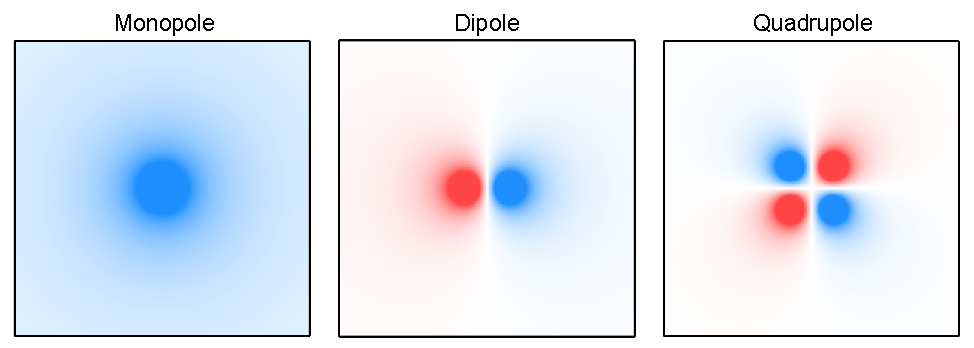
\includegraphics[width=88mm]{Figures/chapter1/multipole_expansion.pdf}
\vspace{-22pt}
\caption{\textbf{The first three terms of the multipole expansion.}}  \label{fig:multipole}
\end{wrapfigure}

The potential due to all current sources and sinks in a medium can be expressed as a so-called multipole series expansion \cite{Nunez2006}. The first term summarizes the \textit{monopole} contributions, which are the contributions of all isolated sources and sinks. The current monopole corresponds to the net flow of current into or out of a volume and is equal in all directions. The second term is the contributions from current \textit{dipoles}, which are paired sources and sinks of equal magnitudes separated by an infinitesimal distance. Due to this specific arrangement, the currents cancel out and thus the dipole has no net monopole moment. The dipole instead expresses the directionality of current flow. The third term is the \textit{quadrupole} contribution. Analogous to the dipole, the quadrupole is the arrangement of four currents that together have no monopole nor dipole moment. These first three terms of the multipole expansion are illustrated in \autoref{fig:multipole}. 

The contribution of each pole to the electric potential decreases with distance at a different rate \cite{Nunez2006}. Specifically,
\begin{equation*}
    \phi(R) = \frac{C_{monopole}}{R} + \frac{C_{dipole}}{R^2}  + \frac{C_{quadrupole}}{R^3}  + \dots
\end{equation*}
The sources and sinks of current are balanced throughout the brain and thus for electric fields generated by macroscopic volumes of tissue, the monopole term is approximately zero \cite{Nunez2006}. Furthermore, for electrodes far away from the current densities, as is the case for EEG, the higher orders terms contribute negligibly relative to the lower order terms. Consequently, EEG signals can be accurately modelled based on current dipoles alone \cite{Nunez2006,RevModPhys.65.413}. This gives us the following equation for the EEG signal \cite{RevModPhys.65.413}
\begin{equation} \label{eq:lead_solution}
    \phi_i(t) \approx \int_V \mathcal{L}_i(\bm{r}) \cdot \bm{Q}(\bm{r},t) dV(\bm{r})
\end{equation}
where $\bm{Q}$ is the current dipole moment at point $\bm{r}$ in the brain. 

\begin{figure}[b!]
    \centering
    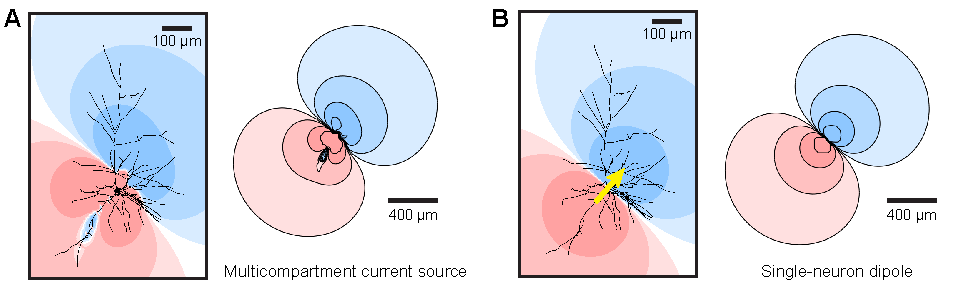
\includegraphics[width=\textwidth]{Figures/chapter1/single_neuron_dipole.pdf}
    
    \caption{\textbf{Single dipole approximation to the electric field generated by an individual neuron.} 
    (\textbf{A}) A multicompartment biophysical neuron model is simulated while receiving synaptic input. The left panel depicts the electric field surrounding the neuron at a moment in time. The right panel is the same simulation zoomed out twice as far (note the scale bars). Red and blue colours indicate positive and negative electric potential, respectively. (\textbf{B}) The electric field is modelled using a single dipole placed at the soma of the neuron (yellow arrow). The single-neuron dipole approximation does not capture the complexity of the electric field near the neuron, but provides a good approximation at further distances.} 
    \label{fig:single_dipole}
\end{figure}

Current dipoles can be modelled at multiple scales. Early work tended to model a neural mass with a single dipole ``mesosource'' that summarized the parallel alignment and synchronous activity of many current dipoles in a volume of neural tissue \cite{Nunez2006}. However, as knowledge grew about the role ionic conductances play in a neuron's electrical properties \cite{Baxter1991}, in tandem with expanding computational power \cite{Beeman2013}, more detailed biophysical models emerged of the current dipoles generated by individual neurons \cite{Murakami2002, Murakami2003 ,Murakami2006, Jones2007}. This led to the idea of a single-neuron dipole \cite{Næss2021,Pettersen2012}. While the morphology and distribution of currents strongly impact the extracellular electric field locally, far from the neuron, the totality of transmembrane currents can be approximated by a single dipole vector centered on the neuron (\autoref{fig:single_dipole}). The use of single-neuron dipoles in EEG modelling is a relatively recent development that provides a level of detail between mesoscopic dipoles, which reflect synchronized neural volumes, and microscopic current sources and sinks, which describe the detailed spatial distributions of transmembrane currents across a neuron. Single-neuron dipoles will play an important role in the modelling work of \autoref{sec:natcomms} and \autoref{sec:apEEG}.

\subsection{Head models of volume conduction} \label{sec:head_models}
After describing the distribution of current dipoles in the brain, the second part to modelling EEG signals comes from defining the lead field, $\mathcal{L}_i(\bm{r})$, at each point in the brain. This lead field must take into account the distribution of conductivity, $\sigma(\bm{r})$, so that the effects of volume conduction are properly modelled. The assumptions that go into calculating $\mathcal{L}_i(\bm{r})$ are together called a head model, i.e., a model that encapsulates all the effects of the head on volume conduction.

The simplest head model is to assume that we are measuring the electric potential inside an infinite, homogeneous volume conductor. Under this assumption, the electric potential at a point $\bm{r}^\prime$ generated by a dipole at a point, $\bm{r}$, is given by
\begin{equation}
    \phi(\bm{r}^\prime) = \frac{\bm{d} \cdot \bm{Q}(\bm{r})}{4\pi\sigma |\bm{d}|^3}
\end{equation}
where $\bm{d}=\bm{r}^\prime-\bm{r}$. This equation should be recognizable as it is very similar to Coulomb's law for the electric field generated by static charges. This model is fairly reasonable for modelling the local field potential (LFP) \cite{Pettersen2012}, but it is a gross simplification for modelling EEG, as it neglects the large differences in conductivity between different tissues.

To capture this variation in conductivity, a popular model is the concentric spheres model. Under this model, the head is composed of concentric spherical layers of different radii and conductivity \cite{Geisler1961}. In the most accurate, four-sphere model \cite{Hosek1978}, the layers represent from inside out: the brain, cerebrospinal fluid, skull, and scalp. The major benefits of these models are that they (i) are more accurate than the infinite, homogeneous volume conductor model, and (ii) can be solved analytically, although the solutions are mathematically and notationally complex. A complete derivation and numerically validated solution to the four-sphere model is given by Næss et al. \cite{Næss2017}.

The most accurate models rely on numerical solutions to the Poisson equation (\ref{eq:poisson}) using techniques such as the finite element method. In this method, the problem domain is meshed into discrete ``elements'' on which the solution is approximated with simple basis functions \cite{Liu2014}. In head modelling, this typically requires representing the various tissues of the head with a mesh of tetrahedral elements, each of which may have its own conductivity value \cite{Hallez2007} (\autoref{fig:FEM_mesh}{A}). Creating a head model for every subject in an experiment would require collecting MRI scans and defining a unique mesh for each subject, and is computational intensive and impractical. Therefore, head models are typically based on the scan of a representative individual \cite{Holmes1998}. An improvement over this was introduced with the the New York Head model \cite{Huang2016}. In this model, Huang et al. \cite{Huang2016} constructed a mesh for the ICBM152 anatomical template, which is an average MRI of 152 subjects, and included different conductivity values for six different tissue types: scalp, skull, cerebrospinal fluid, gray matter, white matter, air cavities (\autoref{fig:FEM_mesh}B). Because this model represents an average head, the lead fields calculated by the model are proposed to be more generalizable than those calculated from a single representative individual \cite{Huang2016}. The New York head model comprises lead fields, $\mathcal{L}_i(\bm{r})$, for 231 electrode locations ($i\in\{1,2,...,231\}$) and for  ${\sim}75000$ cortical locations ($\bm{r}\in\{ \bm{r}_1, \bm{r}_2, ..., \bm{r}_{74382} \}$). These lead fields can be precomputed and stored, thus allowing high accuracy solutions to the forward EEG problem with low computational costs.

\begin{figure}[t!]
    \centering
    \includegraphics[width=\textwidth]{Figures/chapter1/head_models.pdf}
    
    \caption{\textbf{Head models using the finite element method.} 
    (\textbf{A}) Example triangular mesh of a coronal section of the head used for finite element modelling. Figure adapted from Hallez et al. \cite{Hallez2007} under a Creative Commons license. © 2007 Hallez et al; licensee BioMed Central Ltd. (CC BY 2.0).
    (\textbf{B}) Segmentation of the New York head model into six tissue types: scalp (\textbf{a}), skull (\textbf{b}), cerebro-spinal fluid (\textbf{c}), gray matter (\textbf{d}), white matter (\textbf{e}), and air cavities (\textbf{f}). The location of 231 electrodes are shown on the scalp in panel (a). Figure adapted from Huang et al. \cite{Huang2016} under a Creative Commons license. © 2016 Huang et al (CC BY 4.0).
    } 
    \label{fig:FEM_mesh}
\end{figure}

\section{The standard model of EEG} \label{sec:standard_model}

\begin{wrapfigure}[14]{r}{85mm}
\vspace{-20pt}
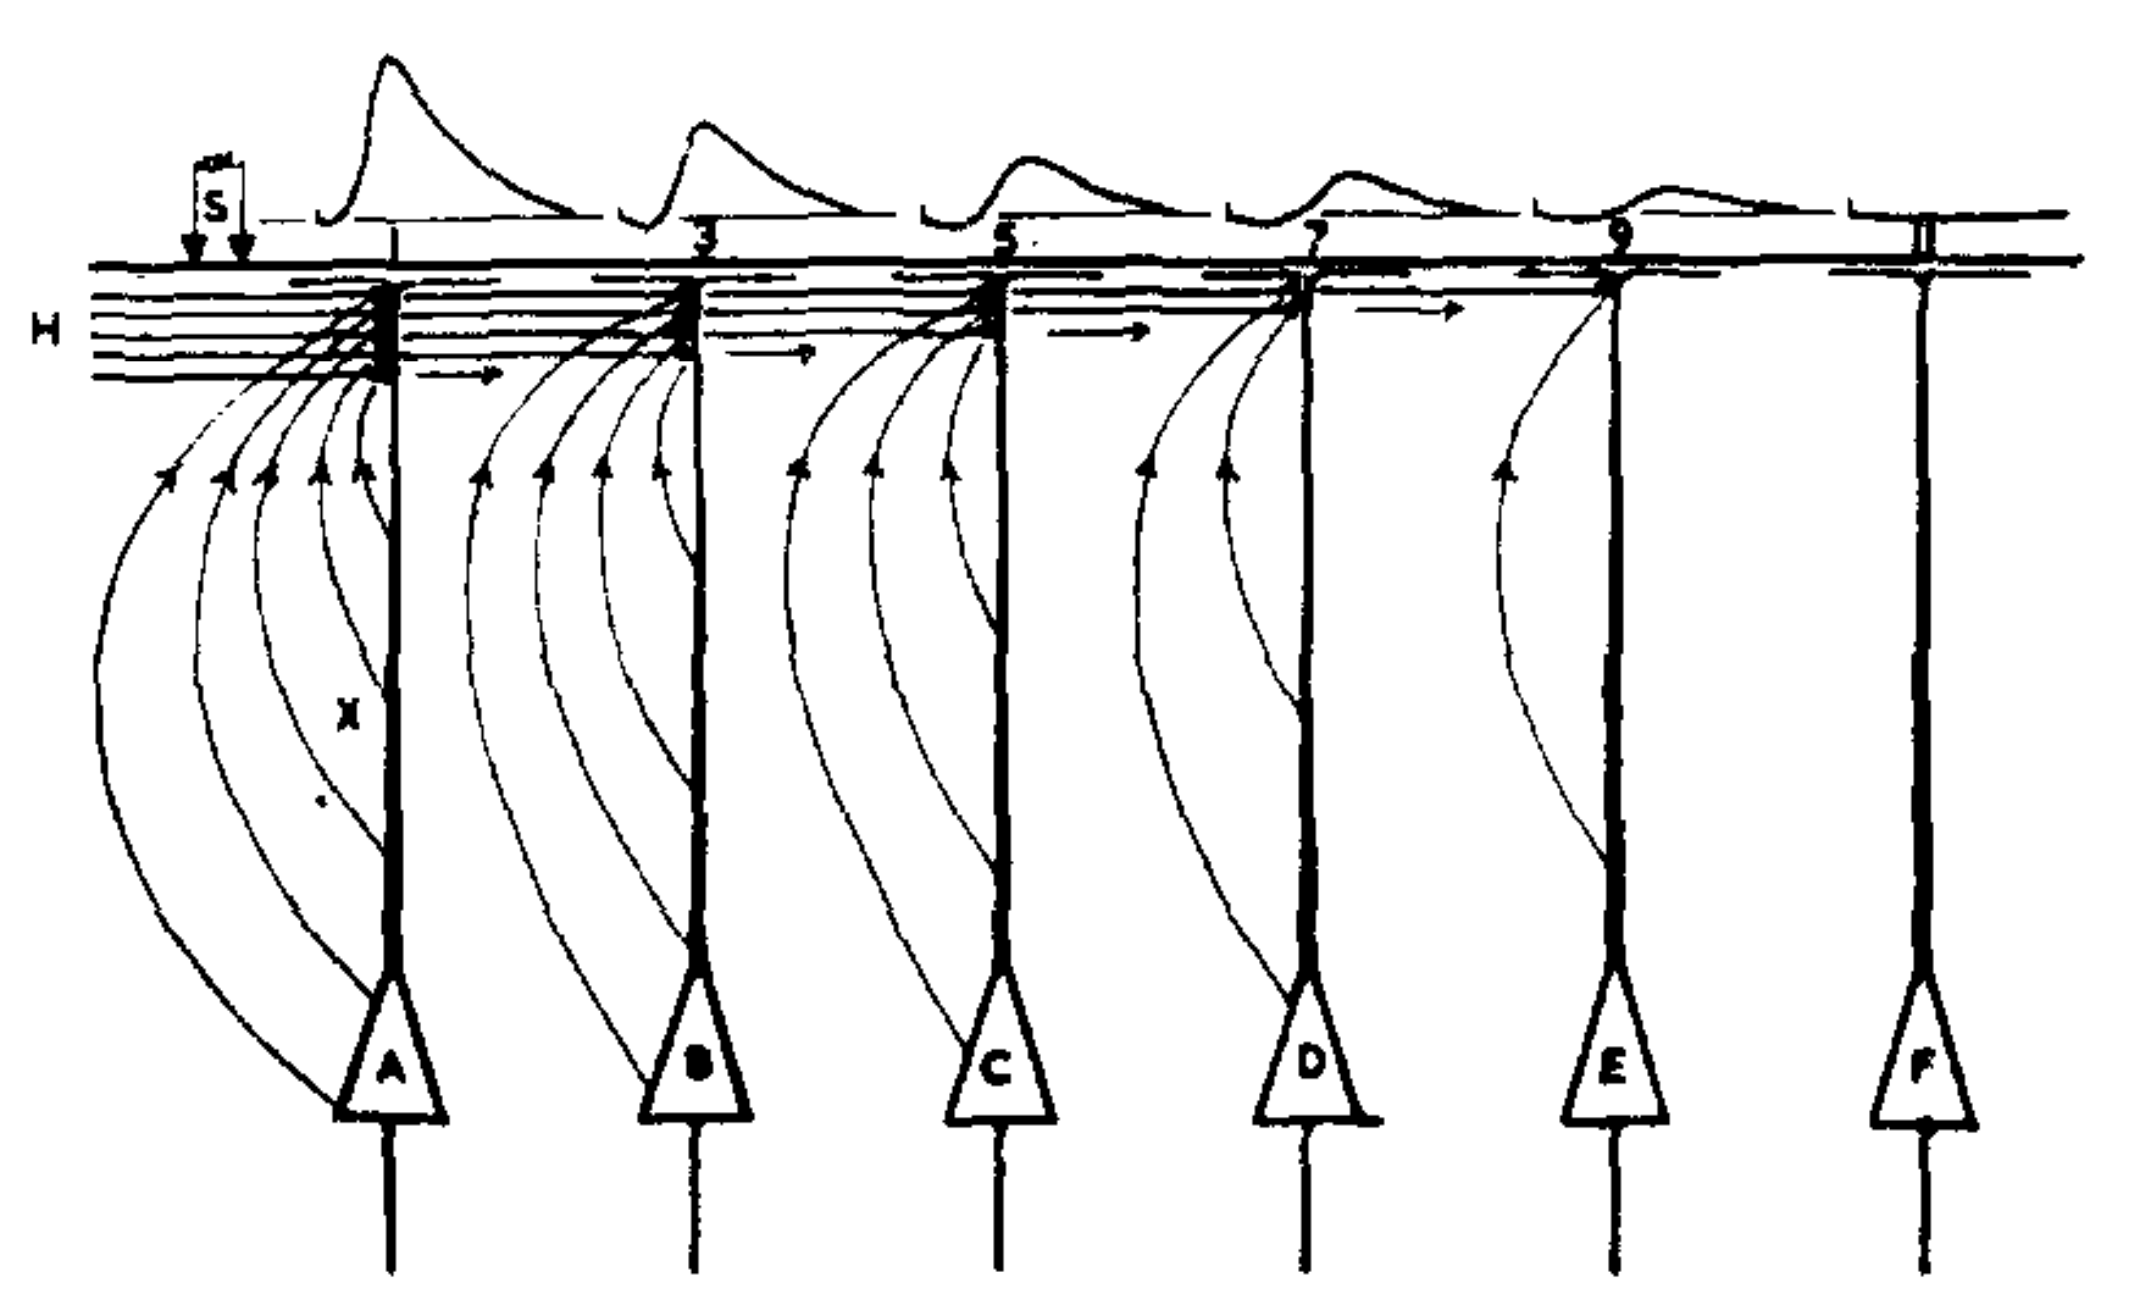
\includegraphics[width=80mm]{Figures/chapter1/Eccles_1951.png}
\caption{ \captiontitle{Early model of EEG generation by Eccles (1951).} Spreading excitation of the apical dendrites of pyramidal neurons generates open field configurations that are aligned in parallel. Reprinted from Electroencephalography and Clinical Neurophysiology, Vol 3/4, J.C. Eccles, Interpretation of action potentials evoked in thecerebral cortex, Pages No. 449-464, Copyright (1951), with permission from Elsevier.
} \label{fig:eccles}
\end{wrapfigure}

The foregoing overview explains how currents in neural tissue produce scalp potentials, but not why the brain generates EEG signals. In addition to the biophysics of EEG, there are two key neural features important for EEG generation: geometry and dynamics. In order to generate electric fields large enough to be detected at the scalp, ion channels must be generating current dipoles that are coherent \cite{Buzsaki2012, Nunez2006}, and because dipoles are vectors, this means that both the temporal dynamics and the spatial configuration of these dipoles must be correlated. The following description reflects the standard textbook explanation of EEG. I say this because some of the theories about the EEG spectral trend to be discussed do not follow this textbook explanation.

\subsection{Pyramidal cells and synaptic currents}

Based on early experimental observations of how superficial potentials propagate following cortical simulation, mid-century electrophysiologists \cite{Eccles1951} reasoned that the EEG signal is likely generated by excitatory synaptic inputs onto the apical dendrites of pyramidal neurons (\autoref{fig:eccles}). This was controversial at the time, as others still believed that the signal primarily reflected action potentials \cite{Burns1950}. It was later confirmed through cross-correlation analysis that postsynaptic potentials and the EEG signal are statistically related \cite{KLEE1965}. Broadly, the synaptic current model became the canonical viewpoint and notably provides both of the necessary mechanisms for EEG generation: (i) synaptic currents last longer than action potential and therefore overlap more in time, which increases the chance of a superposition of current dipoles; and (ii) because of the parallel orientation of pyramidal neurons, synchronized synaptic input into their apical dendrites should generate similarly oriented dipoles.

Early work debated how much EEG signals reflected excitatory versus inhibitory postsynaptic potentials \cite{Pollen1964,Creutzfeldt1966, Creutzfeldt1966a}. It is typically thought that inhibitory synapses are primarily concentrated on the soma \cite{Telenczuk2020, Mazzoni2015,Næss2021}, where transmembrane currents generate small current dioples \cite{Ahlfors2015}. Furthermore, the reversal potential of GABA receptors is closer to the resting membrane potential of the cell, and it has thus been argued that they do not generate as large currents \cite{Buzsaki2012}. However, more recent experimental observations show that neither of these arguments are entirely true. Firstly, inhibitory cells do in fact target the apical dendrites of cortical pyramidal neurons \cite{Palmer2012}. In fact, recent whole-cell synapse mapping shows that inhibitory synapses are more or less uniformly distributed across the entire dendritic arbour \cite{Iacaruso2017}, although still highly concentrated on the soma. Secondly, in vivo neurons are constantly bombarded by excitatory and inhibitory synaptic input, meaning that their membrane potential is not at rest as it is in vitro \cite{Destexhe2003}. The driving force of GABA and AMPA receptors during this high conductance state is much more balanced than seen in experiments in vitro. It is generally considered now that both excitatory and inhibitory synaptic currents contribute to EEG signals \cite{Buzsaki2012}. Nonetheless, many studies of network dynamics still only consider the excitatory synaptic currents when modelling the EEG signal \cite{Jensen2005,McCarthy2008}, and the relative contribution of these two types of currents to EEG signals is far from established. In sum, although every transmembrane current contributes to extracellular potentials, typically only currents mediated by AMPA (and sometimes GABA) receptors are considered as the generators of EEG rhythms.

\subsection{Synchrony through rhythmicity}
If neurons all fire randomly, their electric fields would not sum together in any appreciable way and no EEG signal would transpire. Enter brain rhythms. Neurons are fundamentally oscillators \cite{HODGKIN1952} and oscillators like to synchronize \cite{Strogatz2015}. In fact, it is often difficult to \textit{stop} coupled oscillators from synchronizing \cite{Erb1992}. It is perhaps not surprising therefore that the brain exhibits synchronized oscillations of neurons. These oscillations in turn produce synchronized postsynaptic currents in large pyramidal cells, giving rise to detectable oscillations on the EEG. This is the so-called ``standard model'' of EEG \cite{Cohen2017}. However, there is nothing standard about the wide range of frequencies, neural assemblies, and synchronizing mechanisms that characterize the repertoire of neural oscillations observed in the brain.

The first brain rhythm that was observed was the alpha rhythms (8 to \qty{12}{\hertz}) \cite{Berger1929}, which appears during idleness \cite{Adrian1934}; however, the rhythm may in fact reflect an active inhibition of non-task relevant cortical areas \cite{Cooper2003}. The next rhythms that became apparent are those that are observed during sleep \cite{Loomis1937,Weber2016} and general anesthesia \cite{GIBBS1937,Akeju2017}. Both states share the appearance of delta oscillations ($<4$ \unit{\hertz}), although this rhythm may be caused by distinct underlying mechanisms in sleep and anesthesia \cite{Akeju2017}. Then, there are the rhythms that have been linked to information processing and cognition in awake, behaving humans, including the beta (15 to \qty{30}{\hertz}) \cite{Spitzer2017} and gamma rhythms (30 to \qty{50}{\hertz}) \cite{JASPER1938,Fries2009}. While alpha, beta, delta, and gamma rhythms are perhaps the most notable, there are in fact many more rhythms that have been observed and which span almost the entire frequency range from \qty{0.1}{\hertz} up to \qty{600}{\hertz} \cite{Penttonen2003}. To highlight the diversity in neural rhythms, I will briefly review the neural mechanisms thought to underlie just two of these rhythms: the delta rhythm during sleep and the gamma rhythm observed during wakefulness.

\subsubsection{Example 1: delta rhythms} \label{sec:delta}
Delta rhythms are an intrinsic oscillation of thalamocortical neurons. When these neurons are hyperpolarized to levels below $-65$ to $-70$ \unit{\milli\volt} in vivo, the cells switch from a tonic firing to a bursting regime with a frequency between 0.5 and \qty{4}{\hertz} \cite{Dossi1992}. This bursting activity is characterized by subthreshold oscillations reflecting the interplay of a non-inactivating, hyperpolarization-activated inward current, the h-current, and a low-voltage activated calcium current, the t-current \cite{McCormick1990,Soltesz1991}. These thalamocortical neurons make reciprocal connections with the inhibitory reticular thalamic neurons and this population-level negative feedback is thought to synchronize the oscillations of each thalamocortical neuron \cite{Steriade1991, Steriade1993}. In the waking state, input from the active cholinergic system depolarizes the membrane potential of thalamocortical neurons out of the range of bursting and prevents delta oscillations \cite{Steriade2003}. However, during non-REM sleep, the acetylcholine system is suppressed \cite{Watson2010}, and the resulting lack cholinergic input from the brainstem is thought to let thalamocortical neurons fall into their bursting regime \cite{Steriade2003}. Ultimately, this thalamocortical rhythm produces synchronized excitatory synaptic currents in the cortex, giving rise to the delta oscillations on the EEG during non-REM sleep \cite{Amzica1998}.

\subsubsection{Example 2: gamma rhythms}
 Gamma rhythms have been most completely described in the hippocampus and visual cortex, where it can be evoked by spatial exploration \cite{Bragin1995} and visual attention \cite{Gray1989}, respectively. Unlike the delta rhythm explained above, the gamma rhythm is not an intrinsic property of the constituent neurons. Also unlike the delta rhythm, the gamma rhythm is generated entirely intracortically \cite{Gray1989} and can be examined in vitro using acute cortical slices \cite{Whittington1995}. Such slice work revealed that, mechanistically, gamma oscillations only require a population of reciprocally connected interneurons receiving sufficient excitatory drive \cite{Whittington1995, Buzski2012b}. Indeed, blocking GABA\textsubscript{A} receptors universally prevents gamma oscillations in slices \cite{Bartos2007}. Computational modelling validated that networks comprised entirely of interneurons can synchronize into a gamma rhythm \cite{Wang1996}. It was thus argued that interneuron gamma oscillations create coherent, subthreshold oscillations in pyramidal neurons that in turn synchronize their excitatory outputs, leading to a gamma oscillations on the EEG \cite{Wang1996}. There is also a model of gamma oscillations that requires excitatory connection, the so-called E-I model, as opposed to the foregoing I-I model \cite{Buzski2012b}. In this model, oscillations are generated by alternating excitatory firing followed by delayed reciprocal inhibition \cite{Borgers2003}. This model is also supported by experimental evidence. For example, depending on the pharmacological intervention used to excite interneurons in a slice, blocking AMPA receptors can also prevent gamma oscillations \cite{Bartos2007}. Regardless of the model, it is agreed that gamma oscillations emerge from the local interactions among cortical neurons and that the rhythm's frequency is determined by the timescales of inhibitory currents \cite{Bartos2007, Buzski2012b}.

\subsection{Summary}
In the standard model, EEG reflects populations of excitatory neurons that are entrained to an oscillation. This oscillation synchronizes postsynaptic excitatory currents in pyramidal cells, thus generating widely correlated current dipoles. The mechanisms that produce synchronous oscillations in neurons are diverse and the spatial scale over which this synchrony is exhibited can vary from patches of the cortex to the entire thalamocortical system. The standard model focuses on EEG rhythms and does not provide an obvious explanation for the EEG spectral trend.

\section{Existing theories on the spectral trend} \label{sec:theories}

\subsection{Theory 1. Local versus global synchrony: the classical view} \label{sec:all_oscillations}

The first theory on the EEG spectral trend follows in the tradition of the standard model of EEG and argues that, as EEG reflects brain rhythms, the spectral trend must reflect a particular organization of brain rhythms; the brain does not produce broadband EEG signals, but rather a broad and continuous range of oscillatory signals. According to this theory, the slope of the EEG spectrum is a conflated measure of many different brain rhythms and is not a unified feature of EEG. Instead, EEG spectra appear to exhibit $1/f$ scaling for the following reasons.

\begin{wrapfigure}[9]{T}{65mm}
\vspace{-10pt}
\centering
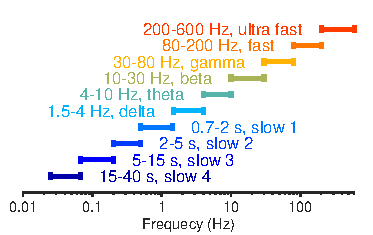
\includegraphics[width=60mm]{Figures/chapter1/rhythm_frequencies.pdf}
% \vspace{-5pt}
\caption{\textbf{The progression of neural oscillations described by Pentoonen and Buzsáki}\cite{Penttonen2003}.}  \label{fig:osc_prog}
\end{wrapfigure}

First, the brain exhibits a wide and diverse repertoire of oscillations that spans a large frequency range. On the lower end of the frequency scale, slow $<1$ \unit{\hertz} EEG oscillations are apparent during sleep \cite{Achermann1997}. On the other end of the scale, ultra-fast oscillations from 200 to 600 Hz were found in the local field potential of the somatosensory cortex of sleeping rats \cite{Kandel1997}, and also appear in human EEG, particularly in patients with epilepsy \cite{Frauscher2017}. In fact, a systematic review found brain oscillations that cover the entire range of frequencies between these two extremes \cite{Penttonen2003}. Moreover, on a logarithmic frequency scale, it was found that oscillations provide continuous and linearly spaced coverage with little overlap (\autoref{fig:osc_prog}). For example, lower frequency oscillations, such as delta rhythms which range from $\sim$1.5-4 Hz, cover a range of a couple hertz, whereas high frequency oscillations, ranging from 200 to 600 Hz, cover a range of several hundred \cite{Penttonen2003}. 

Second, it is argued that slower oscillations recruit larger assemblies of neurons than faster oscillations \cite{Buzsaki2006, Buzsaki2012c, Buzsaki2010}. This argument is based on a theory of temporal coding, the concept that neurons, or assemblies of neurons, encode information through the precise timing of action potentials. Due to conduction delays, it is argued that communication among spatially broad ensembles of neurons must have more tolerance in signal timing (``obtaining a global consensus takes more time'' \cite{Buzsaki2006}), and are therefore organized into slower oscillations. On the other hand, local processing has short conduction speeds and can therefore be more temporally precise and are organized into faster oscillations. During cognitive tasks requiring multiple brain regions, it was shown that long range coherence among EEG channels indeed appeared at lower frequencies \cite{Sarnthein1998,VonStein1999}, whereas LFP and unit recordings have revealed fast, local gamma synchrony among primary visual neurons upon visual stimulation in monkeys and cats, which is believed to be related to local processing in the visual cortex \cite{Gray1989,Eckhorn1994}.

Third, volume conduction acts as a spatial low-pass filter \cite{Nunez2006} and therefore EEG signals are biased by neural activity that is coherent over larger regions of the cortex. In other words, the temporal frequencies characteristic of large spatial scales will be amplified in EEG. In conjunction with the arguments in the foregoing paragraph, one should expect an EEG signal that is dominated by widely synchronized, slow oscillations, while faster oscillations, even if they are widespread, are only locally synchronized and therefore contribute significantly less. Extrapolating this argument to the entire continuum of oscillations described by Pentoonen and Buzsáki \cite{Penttonen2003} and one would expect to see an EEG spectrum which decays linearly in amplitude on a logarithmic frequency scale, essentially giving given the appearance of a 1/f trend.

Adding to these phenomena is the argument that EEG spectra tend to be averaged over many trials or calculated over long periods of time (e.g., \qty{86}{\min} in \autoref{fig:phenomenology}B). However, the state of the brain is constantly evolving and the various rhythms come and go. Therefore, computing EEG spectra over long periods of time, multiple individuals, or different tasks produces spectra that have no clearly obvious peaks as these distinct rhythms have blured together into a continuous spectrum \cite{Buzsaki2006}.

\subsubsection{Caveats}
A drawback to this theory is that, while many oscillations have clearly been found in the brain, there is scant evidence that they are all working together at the same time in healthy, waking and behaving humans. For example, many of these slow oscillations have only been described in sleeping or anesthetized states \cite{Hromadka2013}. Even in a recording of a couple minutes in awake humans, it is unclear why such rhythms mights manifest. Moreover, there is direct evidence, at least in LFP data, that broadband signals do in fact exist; Ray and colleagues showed that increases in the high gamma frequency ranges (80-150 Hz) following visual stimulation is a direct reflection of broadband spiking activity and not rhythmic activity \cite{Ray2008,Ray2011}. 

Furthermore, the central tenet that fast oscillations are locally synchronized and slow oscillations are globally synchronized, while supported by some evidence, still lacks the type of robust experimental observations required to argue this point as a fundamental operating regime of the cortex \cite{Buzsaki2006}. For example, during sleep, it was shown that slow wave oscillations are synchronized over large regions (at least 7 mm), whereas faster oscillations are more locally coherent, with their spatial correlations decaying over just a couple of millimeters \cite{Destexhe1999}. However, faster oscillations were also sometimes observed to be synchronized over 7 mm as well, indicating that there are neural mechanisms for spatially extended synchrony of fast oscillations \cite{Destexhe1999}. Conversely, under propofol anesthesia, the brain exibits slow delta oscillations, but these oscillations are only locally synchronized across less than \qty{4}{\milli\meter} \cite{Lewis2012}. Overall, while there is circumstantial evidence that rhythm frequency is inversely proportional to the size of the neuronal pool, there has been no quantification of this phenomenon per se and it is unclear whether this concept can actually explain the EEG spectra trend quantitatively.

\subsubsection{Summary}
In summary, while this holistic theory of brain oscillations likely explains in part the 1/f appearance of EEG spectra, especially when spectra are averaged over long periods of time, its foundational doctrines still lack some necessary experimental evidence. It also does not provide a clear answer to how the EEG spectral trend should be dealt with. Buszaki, a proponent of this theory, suggests that EEG spectra can be whitened to remove the apparent 1/f trend \cite{Buzsaki2006}. However, if all the power is indeed due to oscillations, it is unclear why this is detrending procedure should be applied at all. Broadly, this theory questions the utility of measures like the spectral exponent. Therefore, if one wishes to claim that the spectral trend provides novel insights complementary to the traditional analysis of EEG rhythms, this is the theory to beat.

\subsection{Theory 2. Self-organized criticality: evidence and controversy} \label{sec:SOC}

Historically, the primary opponent to the above classical view is the theory of self-organized criticality, an alternate model of brain function that invokes a theory developed to explain the ubiquity of power law scaling in nature. Of all the theories reviewed here, that of self-organized criticality is perhaps the most elaborated, controversial, and passionately stated. This passion might partially be due to its proponents viewing power laws with a ``vague and mistakenly mystical sense of universality'', to quote Stumpf and Porter’s perspective piece in \textit{Science}\cite{Stumpf2012}, and is certainly due in part to the theory’s genuinely elegant implications for brain function, such as optimizing dynamic range \cite{Kinouchi2006} and information transmission \cite{Shriki2016}. Like the theory in \autoref{sec:all_oscillations}, the idea of self-organized criticality is principally a theory about brain function, but has also been used to explain the apparent broadband signals in macroscopic neural recordings. 

Many systems appear to exhibit power-law scaling, from earthquakes to forest fires to the stock market. Forty years ago, a now seminal paper by Bak et al. \cite{Bak1987} proposed an explanation for this seemingly universal phenomenon. It was known in statistical physics that systems at second-order phase transitions exhibit power-law scaling in both time and space \cite{pathria2016statistical}. But the parameter regime of this phase transition is infinitesimally small; how could systems everywhere be perched at this delicate point? The theory of self-organized criticality illustrates that certain systems spontaneously tend towards this critical point, by virtue of the complex interactions of the system's constituents, i.e., the critical point is a stable state of the system. Bak et al. \cite{Bak1987} exemplified this with a simple cellular automaton model. Cells are laid out in a lattice and each is associated with a number value. If a cell’s value exceeds a threshold, then a value of one is transferred from the cell to each of its neighbors. When initializing values randomly, the system will eventually settle into an equilibrium state, but one which is extremely sensitive to perturbation. Tripping just one of the cells will send off a so-called ``avalanche'', whose size, $S$, was shown to be distributed as a $1/S^\beta$ power law. In his book, \textit{How Nature Works}\cite{Bak1996}, Per Bak argues that ``the complex phenomena observed everywhere indicate that nature operates at the self-organized critical state.''

The parallels between the original cellular automaton model and neural networks are quite apparent. When a neuron’s excitatory input reaches a certain threshold, the cell fires an action potential, which causes an excitatory potential in each of the cell’s postsynaptic partners (assuming all neurons are excitatory). Consequently, there was much early interest among physicist in applying the theory of self-organized criticality to the brain \cite{Corral1995, Herz1995}. While these original studies on simulated neural networks needed to tune parameter values to achieve a critical process, it was later shown that a network of excitatory integrate-and-fire neurons will self-organize into a critical state with the addition of synaptic depression \cite{Levina2007}. It was also shown that networks of excitatory and inhibitory integrate-and-fire neurons exhibit avalanche criticality when excitation and inhibition is particularly balanced \cite{Poil2012, Lombardi2017}. In brief, there were many early studies suggesting that self-organized criticality is theoretically possible in neural networks.

Accordingly, it was also suggested that self-organized criticality underlies the power-law scaling observed in macroscopic neural recordings \cite{Lombardi2017}. Indeed, the average height, $S$, of an avalanche is related to its duration, $T$, as $S(T)\propto T^{1/\sigma\nu z}$, with the consequence that the system's spectrum should also follow a power-law \cite{Kuntz2000} (the exact meaning of the parameters $\sigma$, $\nu$, and $z$ are not relevant for our discussion but are defined by Kuntz and Sethna \cite{Kuntz2000}). It has been shown that simulated networks of excitatory and inhibition neurons at criticality generate neuronal avalanches with a spectral exponent $\beta\in[1,2]$ depending on the percentage of inhibitory syanpses in the model \cite{Lombardi2017}. So what evidence is there that the brain is actually operating in a self-organized critical state?

At the turn of the millennium, Beggs and Plenz \cite{Beggs2003} tested whether slices of brain tissue exhibit cascades of action potentials that obey the dynamics of a self-organized state. Organotypic and acute slices were studied on an electrode array and negative deflections at each electrode, indicative of locally synchronized spiking, were analyzed. These experiments were the first to show that cortical circuits can exhibit so-called neural avalanches – cascades of activity with sizes and durations that obey power laws. Indeed, it was found that the activity was consistent with a branching process (see \hyperref[box:first]{Box 1}). Later, neuronal avalanches consistent with a branching process were also identified in LFP recordings in monkeys in vivo, indicating that this phenomenon may indeed play a role in physiological brain dynamics \cite{Petermann2009}. Power-law relations have since been identified across many species using many different recording modalities, including voltage \cite{Scott2014} and calcium imaging \cite{Bellay2015,Ponce-Alvarez2018}.

\begin{mybox}[floatplacement=t,label={box:first}]{Definition of branching process}
   A \textit{branching process} describes the evolution of a population of individuals, whereby at the end of a generation, each individual dies and leaves behind a certain number of offspring. In a neural network, these individuals are taken to be action potentials and the offspring are the subsequent action potentials elicited in postsynaptic partners. The dynamics of a branching process are determined by the branching number, $m$, which reflects the average number of offspring per individual. Branching processes are often modelled with immigration, that is at each generation a number of individuals, $h$, are added to the population in addition to the offspring. Mathematically, the population size at a given time point, $A_t$, is given by the following recursive equation \cite{Wilting2018}
    \begin{equation}
        A_{t+1} = \sum_{i=1}^{A_{t}} y_{i,t} + h_t
    \end{equation}
    where $y_{i,t}$ is the number of offspring for individual $i$ of generation $t$.  $y_{i,t}$ are independent and identically distributed according to some law $y_{i,t}\sim\mathcal{Y}$, with mean $\mathbb{E}(\mathcal{Y})=m$. If the branching number is $m>1$, then the population size, e.g., number of action potentials, will increase exponentially and unbounded. If the branching number is $m<1$, the population size will reach a stable steady-state, $A_{\infty}=h/(1-m)$. Thus, a parameter value of $m=1$ is a critical point of the system. Notably, as $m\to1$, the number of individuals will exhibit avalanches with a size distribution that approaches a power law with a slope of $-3/2$, exactly that observed by Beggs and Plenz \cite{Beggs2003}.
\end{mybox}


\subsubsection{Caveats}

Despite the explosion of papers on self-organized criticality in the brain over the past two decades, the topic remains highly controversial. One caveat to these studies is the lack of strong statistical evidence for power laws. For example, to conclude there is a power law in a probability distribution this relationship should continue over at least two decades of the variable and should be estimated with maximum likelihood estimation \cite{Stumpf2012}. Secondly, there should be an actual statistical test of whether the relationship is best explained by a power law. Only a couple of the foregoing studies performed robust statistical analyses on their avalanche distributions \cite{Clauset2009}. The most convincing analyses are from calcium imaging studies \cite{Bellay2015, Ponce-Alvarez2018}. However, due to the slow kinetics of calcium indicators, the avalanche power spectrum can only be computed for very low frequencies, less than 1 Hz in the case of Ponce-Alvarez et al.\cite{Ponce-Alvarez2018}, and therefore unfortunately do not provide much information on the EEG spectral trend. 

The requirement for a power law over two decades of data is a particularly strong caveat in tying self-organized criticality to EEG, as a look through the literature on EEG spectra reveals a hodge-podge of power law measurements, which typically rely on simple linear regression and are often over short segments of spectra: $\beta=2$ from 30 to 50 Hz \cite{Lendner2020}; $\beta=1.4$ from 0.15 to 9.5 Hz \cite{Dehghani2010}; $\beta=1.3$ from 0.5 to 30 Hz \cite{Pritchard1992};  $\beta=-1$ from 1 to 40 Hz \cite{Colombo2019}; $\beta\in[1,3]$ from 3 to 30 Hz \cite{Pereda1998}. This is by no means an exhaustive list. One likely reason for these varied and often short frequency ranges is the difficulty in estimating power laws from the whole spectrum; EEG spectra clearly exhibit peaks due to narrowband neural activity, and it is unclear how these peaks should be accounted for when measuring purported power laws. These peaks are either entirely ignored and included in the power-law fit (\autoref{fig:phenomenology}A), or the spectra are averaged over such long periods of time that the peaks are blurred to the point of nonrecognition. Even a ``short'' time window of 20 s (as used for validation by He et al.\cite{He2010}; $\beta\in[2,3]$ from 1 to 100 Hz) contains at least 1000 periods of an oscillation above \qty{50}{\hertz}, over which time the oscillation may disappear and reappear or fluctuate widely in frequency. Consequently, there is very high potential for the blurring of spectral peaks, and scaling at these frequencies may therefore be an epiphenomenon of purely rhythmic activity. In fact, such a blurring of spectral peaks at various frequencies is essentially the argument outlined above in \autoref{sec:all_oscillations} and is clearly not consistent with self-organized criticality. Even methods that claim to account for rhythmic EEG components measure different spectral exponents from the same spectrum (\autoref{fig:gerster}).  In sum, the evidence of power-law scaling in EEG spectra is inconsistent and the actual value of the spectral exponent is very poorly defined. 

A second caveat to assessing criticality in the brain is that the nature of in vivo electrophysiological measurements severely undersamples the neuronal population, which prevents accurate inference of power laws and branching numbers \cite{Priesemann2009}. Even imaging studies often only genetically express calcium or voltage indicators in a subset of neurons, such as layer 2/3 pyramidal cells \cite{Scott2014,Bellay2015}. One study was performed in transgenic zebrafish \cite{Ponce-Alvarez2018}; however, despite expressing GCaMP under a pan-neuronal promoter, transgenic expression is often incomplete and highly variable between cells. Therefore, even measurements of ``whole-brain dynamics'' still suffer from subsampling. Recent theoretical advances have provided statistical tools for accurately inferring branching numbers from undersampled systems \cite{Wilting2018}. Applying these statistical tools to in vivo electrophysiological recordings have suggested that the cortex does not operate at criticality, but rather in a subcritical regime, with a branching number calculated to be between 0.95 and 0.998 \footnote[2]{This might not seem far off from $m=1$. However, as pointed out by Wilting and Preisemann\cite{Wilting2019}, the susceptibility of the system to external perturbation is $\partial A/\partial h = \frac{1}{1-m}$, which means the overall dynamics are extremely sensitive to small differences in the branching number around the singularity.} in monkeys, cats, mice \cite{Wilting2018,Wilting2019} and zebrafish \cite{Suryadi2022}. Interestingly, it has been noted that the purported computational properties that are maximized at criticality also come with trade-offs, such as poor reliability \cite{Gollo2017} and critical slowing down \cite{Scheffer2012, Wilting2019a}. Therefore, it has been suggested that a slightly subcritical dynamical regime may in fact balance the various computational tasks of the cortex better than it would at criticality \cite{Wilting2019a}.

A final caveat to this theory is that the EEG signal is not a measure of the average firing rate of a network (\autoref{sec:EM_theory}). Therefore, the spectrum of neural avalanches, or even subcritical dynamics, does not immediately translate into the spectrum of the EEG. None of the studies discussed above attempted to simulate the electric fields potentially generated by their modelled neural networks.  Therefore, as in the previous theory, it is unclear whether this theory quantitatively explains the scaling observed in EEG spectra.

\subsubsection{Summary}

Self-organized criticality is a theory about the dynamical regime in which cortical networks operate, which has been claimed to confer special computational advantages. However, the evidence that the brain operates at a self-organized critical point is controversial. The most statistically sound evidence comes from estimating the branching number (\hyperref[box:first]{Box 1}) from in vivo spike recordings, which has consistently indicated that the brain operates below criticality. What does this all mean for the EEG spectral trend? What is clear from all the above evidence is that the cortex can operate in an aperiodic regime characterized by cascades of neural activity, regardless if these cascades obey a strict power law. This observation casts some doubt on the standard model of EEG, which assumes that all synchronous activity occurs through neural oscillations. Might subcritical network dynamics be capable of generating aperiodic EEG signals? Surprisingly, this simple question has not yet been addressed.

\subsection{Theory 3. Synaptic timescales: unchallenged and underexplored} \label{sec:timescales}

In their paper ``Does the 1/f Frequency Scaling of Brain Signals Reflect Self-Organized Critical States?'', Bedard et al.\cite{Bedard2006} presented an early challenge to the hypothesis that EEG spectra indicate self-organized criticality and proposed an alternate explanation. The authors performed inter-spike interval and avalanche analysis on isolated spikes measured with bipolar extracellular electrodes in waking and sleeping cats, and found that the statistics of spiking were almost perfectly captured by a Poisson process \cite{Bedard2006}. To model the simultaneously measured LFP signal, the authors convolved the recorded spike trains with an exponentially-decaying synaptic response, which generated a spectrum with an exponent of $-2$. The authors argued that the scaling observed in LFP spectra results from the filtering of an essentially white-noise process by the kinetics of postsynaptic potentials. Mathematically, this is expressed quite simply. Because convolution becomes multiplication in Fourier space, the power spectrum of this system is
\begin{equation}
P(f) =|\hat{C}(f)|^2 \frac{\tau^2} { 1+ (2\pi\tau f)^2}
\end{equation}
where $\tau$ is the decay time constant of the synaptic current (which the authors modelled with $\tau=10$ \unit{\milli\second}), and $|\hat{C}(f)|^2$ is the power spectrum of the ``drive'' signal, which in the case of a homogeneous Poisson process will simply be equal to the mean rate. Thus, if macroscopic recordings (LFP and EEG) reflect postsynaptic currents, the timescale of these responses should shape the signals' spectra. Notably, the authors found that their LFP spectra scaled with an exponent of $-3$ above 20 Hz. This ``missing'' 1/f factor was attributed to filtering of the signal through neural tissue (see \autoref{sec:filter_theory} below).

Later Miller et al. \cite{Miller2009} published a similar model for electrocorticographic (ECoG) recordings \footnote[2]{ECoG is similar to EEG but the electrodes are placed on the surface of the dura. It is an invasive recording that measures EEG signals intracranially.}. Spectra averaged over several minutes of data indicated an exponent of $-4$ at frequencies above 80 Hz. They argue, similarly to Bedard et al., that a $1 / (1+ (2\pi\tau f)^2)$ factor is contributed by the decay kinetics of synaptic currents (these authors fit their spectra with $\tau=4$ \unit{\milli\second}), while the additional $-2$ factor was explained in a mathematically similar way, with a leak current that restores the membrane potential with a slow time constant of \qty{100}{\milli\second}.

In short, both papers argue that synaptic currents significantly shape the spectra of macroscopic recordings, but disagree over how much additional filtering is exhibited and what the mechanism underlying this additional filtering may be. There is significant experimental evidence that postsynaptic potentials are the primary sources of LFP and EEG, making the core argument of these papers highly plausible. However, as described in \autoref{sec:standard_model}, experimental evidence largely points to both excitatory and inhibitory currents as sources of EEG signals. It is therefore interesting that both studies only fit their spectra with a single synaptic timescale and moreover that Miller et al. \cite{Miller2009} found a timescale that more closely matches the kinetics of AMPA receptors, whereas the timescale from Bedard et al. \cite{Bedard2006} more closely matches the kinetics of GABA receptors (\autoref{sec:I_syn}).

Gao et al. \cite{Gao2017} were seemingly the first to explicitly consider the scaling imparted by both inhibitory and excitatory currents. The authors modelled macroscopic recordings with the same model as Bedard et al. \cite{Bedard2006}, except that Gao et al. considered two processes, one filtered by inhibitory synapses and another filtered by excitatory synapses. This simple extension led to an important insight. Because these two processes are filtered by different time constants, they contribute to the spectrum in different frequency ranges. In particular, because GABA receptor kinetics are slower than AMPA receptor kinetics, the inhibitory process contributes power preferentially at low frequencies (\autoref{fig:gao}). Consequently, if the synaptic excitation to inhibition (E:I) ratio decreases, e.g., if inhibition increases in amplitude, there will be an increase in the spectrum specifically at lower frequencies. The authors concluded that the synaptic E:I ratio determines the spectral exponent between 30 and 50 Hz, a range determined jointly by the time constants of excitatory and inhibitory synaptic decay (\autoref{fig:gao}).

\begin{wrapfigure}[16]{r}{65mm}
\vspace{-20pt}
\centering
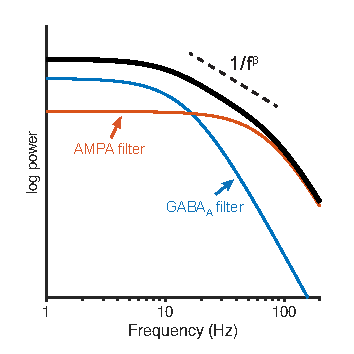
\includegraphics[width=60mm]{Figures/chapter1/EI.pdf}
\vspace{-14pt}
\caption{\textbf{Synaptic timescale hypothesis with excitation and inhibition.} Gao et al. \cite{Gao2017} hypothesized that if macroscopic neural recordings reflect synaptic currents, the signal will be filtered by an AMPA receptor filter (red) and GABA receptor filter (blue). The spectrum of the recording (black) will exhibit a spectral exponent determined by the relative contribution of excitatory and inhibitory currents.}  \label{fig:gao}
\end{wrapfigure}

As described above, there is strong experimental evidence that the macroscopic electric fields generated by the brain reflect primarily postsynaptic currents, making this theory highly plausible. However, this theory does have important caveats. Firstly, all of the studies described above modelled the field as a filtered Poisson process, i.e., there was no synchrony assumed in any of the models. Miller et al.\cite{Miller2009} argued explicitly that the spectral trend reflects ``asynchronous'' brain signals. This is clearly at odds with the standard model of EEG which states that EEG only reflects synchronized brain activity. Secondly, while both inhibitory and excitatory currents are thought to contribute to EEG signals, the relative contributions of the two are not known. To get their result, Gao et al. \cite{Gao2017} chose an E:I ratio that has inhibition contributing  most of the power to the EEG signal, which is also seemingly at odds with the standard model of EEG which emphasizes the role of excitatory currents. Finally, all models used synaptic filtering to explain experimentally measured spectral exponents, but synaptic filtering should impart a very specific shape to the EEG spectrum (\autoref{fig:gao}) which is not a $1/f^\beta$ power law. It has not been shown whether this model actually fits the shape of real spectra across a broad range of frequencies.

\subsection{Theory 4. Frequency dependence of neural tissue} \label{sec:filter_theory}
The next theory discussed here has been argued extensively back and forth, and is desentient yet persistent in the face of the now broadly accepted narrative of tissue properties. In a series of papers, Bédard et al.\cite{Bedard2004, Bedard2006a, Bedard2009} set out to show theoretically that electrical signals measured in LFP recordings are filtered by the extracellular medium. In the first paper, the authors sought to show this by deriving a model from first principles whereby Maxwell’s equations are considered under spherical symmetry, but spatially inhomogeneous conductivity \cite{Bedard2004}, i.e., $\sigma$ in \ref{eq:poisson} is a function of space. Through numerical simulations, this study found that the extracellular medium may act as either a low or high pass filter, depending on the precise spatial distribution of conductivity values. However, the most physiologically realistic distributions of conductivity did not produce any frequency-dependent filtering of the electric field. The model was later elaborated by considering polarizing effects, whereby the electric potentials generated by neural activity polarize the membranes of nearby passive cells, such as glia \cite{Bedard2006a}. These polarized membranes then generate their own ``induced'' electric field. This induced field re-equilibrates as ionic charges redistribute, which occurs with exponentially decaying dynamics. Effectively, this model is similar to the synaptic timescale model, except here, the filter is imparted by the extracellular medium. This model was undermined in a subsequent paper of theirs \cite{Bedard2009}, however, in which the model parameters were constrained by experimental measurements of brain tissue conductivity \cite{Gabriel1996}. These simulations suggested that it is only possible for membrane polarization to filter signals below approximately 1 Hz.

Instead, Bédard and Destexhe\cite{Bedard2006a} introduced ionic diffusion into their model, which added an additional $1/\sqrt{f}$ filter to the signal and was in line with the frequency dependent conductivity values measured by Gabriel et al.\cite{Gabriel1996}. However, prior to this last paper, Logothesis et al.\cite{Logothetis2007} had developed a new setup for measuring brain conductivity in primates in vivo. They argued that because Gabriel et al. \cite{Gabriel1996} had measured conductivity with a single pair of metal plates, ionic diffusion in fact lead to charge accumulation at the electrode-electrolyte interface, which is expected to produce frequency dependent measurement errors \cite{Warburg1899}. By using a four electrode system, the electrode pair used to measure voltage in the experiments of Logothesis et al.\cite{Logothetis2007} was not subject to charge accumulation and therefore did not suffer from confounding frequency-dependent measurement errors. The results indicated that the conductivity of neural tissue is almost entirely independent of frequency in the range relevant for LFP and EEG \cite{Logothetis2007}, an observations that has since been verified by many subsequent studies (reviewed by Pesaran et al.\cite{Pesaran2018}). Nonetheless, Bédard and Destexhe\cite{Bedard2006a} argued that under true physiological conditions, ionic diffusion should still play a role in filtering electric fields due to the redistribution of ions after the activation of ion channels. The exact magnitude with which this phenomenon may contribute under physiological conditions was not quantified.

These studies all focused on LFP recordings and therefore only concerned themselves with the filtering of neural tissue, whereas EEG signals must also pass through the scalp and skull. These structures are reported to have frequency-dependent conductivities, but this filtering is seemingly minor at the frequencies relevant to EEG \cite{Pfurtscheller1975, Akhtari2002, Pesaran2018}. Moreover, differences in this frequency-dependence across individuals seem to be insignificant \cite{Akhtari2002}, and changes in this filtering over time is highly unlikely. No studies have explicitly claimed that the spectral trend in EEG is a result of frequency-dependent filtering of the scalp or skull.

The debate over whether tissue properties can cause 1/f scaling in macroscopic electric measurements is ongoing \cite{Bedard2017}. However, by and large, present evidence suggests that the effects are minimal. Importantly, even if frequency dependent filtering plays a small role in determining the overall scaling of EEG recordings, these filtering effects would not be expected to vary significantly over time or across individuals. Therefore, these mechanisms are unlikely to explain differences, for example task-related changes, in the broadband component of EEG spectra. 

\subsection{Theory 5. Intrinsic dendritic filtering}
A final theory on the spectral trend comes from biophysical simulations of the electric fields generated by single neurons. As background, it is well known that postsynaptic currents in the soma are low-pass filtered versions of the currents at the synapses \cite{Rall1967}. In other words, dendrites act as a low-pass filter of intracellular currents. In a series of papers, Einevoll and colleagues showed that the extracellular potential exhibits spatially dependent filtering as a direct consequence of the intrinsic properties of dendrites. Because the extracellular potential primarily reflects nearby transmembrane currents \cite{Nunez2006}, the extracellular potential recorded near the soma will be a low-pass filtered version of that recorded near the synapse \cite{Linden2010}. In general, the further away one records from the synapse, the more the potential will be determined by transmembrane currents across the entire cell and the potential will therefore adopt more and more of the low-pass filtering imparted by the dendrites \cite{Linden2010}. It was noted by the authors that the $1/f$ factor missing from the synaptic timescale model of Bedard et al. \cite{Bedard2006} could be accounted for by dendritic filtering even in a purely resistive and homogenous extracellular medium \cite{Linden2010,Pettersen2008}. Later, the authors calculated the spectrum of single-neuron dipoles generated by neurons receiving white noise input, finding a spectral exponent of $-3/2$ at asymptotic frequency values \cite{Pettersen2014}. There are no caveats to these findings, per se. However, the interpretation of this filtering mechanism in the context of the synaptic timescale hypothesis is considered in the general discussion (Chapter 4). 

\subsection{The high frequency plateau} \label{sec:plateau}
In addition to the $1/f$ scaling that the foregoing theories attempt to explain, EEG spectra also exhibit a high frequency plateau (\autoref{fig:gerster}), whose origin is not entirely determined \cite{Gerster2022}. This part of the spectral trend has received less attention because EEG analysis is traditionally focused on lower frequencies; however, as noted in \autoref{sec:all_oscillations}, the brain exhibits rhythms at frequencies extending as high as \qty{600}{\hertz}. Moreover, estimates of the spectral trend at lower frequencies can still be affected by this plateau (\autoref{fig:gerster}). Thus, understanding the spectral plateau in EEG is important for obtaining a full picture of the spectral trend. 

The spectral plateau could come from several sources. Obviously, the noise floor of the amplifier will contribute to a plateau if the signal to noise ratio drops too low \cite{Scheer2006}. EEG is also known to reflect electric potentials generated by currents in muscles, which generate broadband signals especially above \qty{30}{\hertz} \cite{Muthukumaraswamy2013}. Neither of these explanation suggest that the high frequency plateau in EEG provides neurophysiological information. However, LFP recordings, which do not pick up muscle signals, exhibit high frequency plateaus in their spectra above the noise floor of the amplifier. It has been suggested that this high frequency plateau is caused by neural activity, such as the high frequency currents of voltage-gated channels during action potentials \cite{Ray2008, Ray2011, Gao2016, Zanos2010}. It has been suggested that this same signal could contribute to high frequency broadband signals in intracranial EEG and possibly even scalp EEG \cite{Ray2008}.

\section{Summary and research rationale}

There exist many competing theories on the mechanisms underlying the EEG spectral trend. Some of these theories challenge the standard model of EEG and state that EEG signals reflect arrhythmic neural activity. If true, these theories suggest that much of the spectral EEG analysis performed over the past decades may be flawed. Others suggest that the EEG spectral trend is an epiphenomenon reflecting a hierarchy of neural oscillation and that the slope of the spectral trend is a conflated measure of brain rhythms. According to this view, researchers should go about analyzing their data as they always have. To do so confidently, the field needs a rigorous assessment of alternate view points.

While all the theories discussed above make predictions about the spectrum of the electric potential, few employed biophysical models of electric field generation. None of the theories attempted to use head models to simulate actual EEG signals. This gap is particularly noticeable in the theory of neural avalanches and the synaptic timescale hypothesis, both of which controversially propose that EEG reflects non-oscillatory neural activity. This assertion needs to be tested with biophysically accurate models of EEG generation.

For each theory whose assumptions are validated, their implications for spectral analysis need to be more concretely determined. Despite the original assertion of Pritchard, only the theory of self-organized criticality suggests that the EEG spectral trend should follow a pure power-law, and even this would not hold if neural activity falls short of actual criticality as the evidence suggests. The other theories broadly explain the spectral trend with various low-pass filtering mechanisms, which produce a power law at asymptotic frequencies but not at low frequencies where most brain rhythms lie. Indeed, from the literature review work done in this chapter, it is clear that the present state of the field already calls into question the practice of removing the $1/f^\beta$ component. Presumably, working out the biophysics of the spectral trend will tell us the most physiologically meaningful method of spectral detrending, if necessary at all.

The core aim of this thesis is to constrain theories on the spectral trend with biophysical laws and experimentally determined physiology. In Chapters 2 and 3, I develop biophysically detailed models to evaluate whether the electric fields generated by synaptic currents and action potentials are sufficiently coherent to be measured by scalp electrodes during various types of aperiodic neural activity. By incorporating experimental work performed by collaborators, the results from Chapter 2 largely validate the synaptic timescale hypothesis and suggest that GABA receptor kinetics significantly shape EEG spectra. Chapter 3 investigates the role of voltage-gated channels in shaping EEG spectra and builds towards a theory for the EEG spectral trend at higher frequency and specifically the high frequency plateau observed there. In each chapter, I investigate the implications of the modelling conclusions for practical spectral analysis, specifically when spectral detrending is appropriate and how it should be performed.